\documentclass{article} % This command is used to set the type of document you are working on such as an article, book, or presenation

\usepackage{geometry} % This package allows the editing of the page layout
\usepackage{amsmath}  % This package allows the use of a large range of mathematical formula, commands, and symbols
\usepackage{graphicx}  % This package allows the importing of images
\usepackage{soul}
\usepackage{amsfonts}
\usepackage{dirtytalk}
\usepackage{tabto}
\usepackage{xcolor,colortbl, amssymb}
\usepackage{forest}
\usepackage[ruled, lined, linesnumbered, commentsnumbered, longend]{algorithm2e}

% https://www.messletters.com/en/big-text/

\newcommand{\question}[2][]{\begin{flushleft}
        \textbf{Problem #1}: \textit{#2}

\end{flushleft}}

\definecolor{Green}{rgb}{0, 1, 0}
\definecolor{Pink}{rgb}{1, .753, .796}

\newcommand{\sol}{\textbf{Solution}:} %Use if you want a boldface solution line
%\newcommand\tab[1][0.4cm]{\hspace*{#1}}
\newcommand{\maketitletwo}[2][]{\begin{center}
        \Large{\textbf{Homework #1}
            
            CMPSC 465} % Name of course here
        \vspace{5pt}
        
        \normalsize{Kinner Parikh  % Your name here
        
        \today}        % Change to due date if preferred
        \vspace{40pt}


        \newpage
        
\end{center}}
\begin{document}
    \maketitletwo[6]  % Optional argument is assignment number
    %Keep a blank space between maketitletwo and \question[1]

    \question[1]{}
    \begin{center}
        
        I worked with Sahil Kuwadia and Ethan Yeung
    
        I did not consult without anyone my group member
    
        I did not consult any non-class materials
    \end{center}
    
    \newpage

    \question[2]{DFS Variations}

    a) To find if there is a feasible path from $s$ to $t$, we can simply run DFS on the graph starting 
    
    at $s$, ignoring all edges whose weight is greater than $L$. Thus, the only edges we can travel are 
    
    those for which $\ell_e \leq L$.

    \begin{algorithm}
        \caption{feasibleRoute}

        \SetKwFunction{feasibleRoute}{feasibleRoute}
        \SetKwInOut{KwIn}{Input}
        \SetKwInOut{KwOut}{Output}

        \KwIn{$G = (V,(E, \ell_e))$ (in adjacency list format), $s$, $t$, $L$}
        \KwOut{A feasible path exists or not}

        Initialize an empty stack, $st$, that will store nodes

        Create visited list for all nodes and set all to false
        
        Push $s$ into $st$

        \While{st is not empty}{
            $x \leftarrow$ pop first element in $st$
            
            \If{x not in visited}{
                add $x$ to visited

                \ForAll{neighbors a of x}{
                    \If{$\ell_a$ $\leq$ L}{
                        \If{a is t}{
                            return True
                        }
                        push $a$ onto stack
                    }
                }
            }
        }
        return False

    \end{algorithm}
    \underline{Proof of correctness}

    Initialization: 

    \hspace{5pt} The stack is initialized with only $s$ at the beginning. This represents the first city you leave 
    
    \hspace{5pt} from, thus the base case holds.

    Maintenance:

    \hspace{5pt} Assuming we are at an arbitrary city $k$, which means that there is a path to $k$ that is valid 
    
    \hspace{5pt} and we know $k$ is the top of the stack, we can pop $k$ off. If $k$ has already been visited, then 
    
    \hspace{5pt} we don't do anything. If it hasn't been visited, then we add $k$ to the visited list and look at 
    
    \hspace{5pt} the cities that are adjacent to $k$. We can iterate through all the cities that are adjacent to $k$, 
    
    \hspace{5pt} and check if the weights on those edges are less than $L$. If they are, then we can push them 
    
    \hspace{5pt} onto the stack. When we push them onto the stack, we know that they are reachable from $k$, 
    
    \hspace{5pt} thus we can check if the adjacent node is $t$, in which case we know that $t$ is reachable, and we 
    
    \hspace{5pt} can return true. If it isn't, we simply continue.

    Termination:

    \hspace{5pt} When the stack is empty, which means that all the reachable nodes have been visited, we can 
    
    \hspace{5pt} confidently say that there is no feasible route from $s$ to $t$ and return False. $\square$

    \underline{Runtime:} Since this algorithm is simply DFS, and all the modifications we make to the 
    
    lgorithm complete in constant time, this will run in $O(|V| + |E|)$.

    \newpage

    b) To find the minimum fuel tank capacity we need to find a path that has the least maximum 
    
    distance. We start by finding all the unique edge distances in the graph. We can go through 
    
    the graph's adjacency list and add all the distances to list $l$, making sure not to add duplicate 
    
    distances into $l$. Once we have all distances, we sort $l$ using merge sort such that all the unique 
    
    distances are increasing in order. We can then call leastMaxDistance using this sorted list.
    
    %Using this sorted $l$, we find the number of entries in the list as $n$. We can use this list to begin performing a binary traversal, starting at index $n/2$.

    \begin{algorithm}
        \caption{leastMaxDistance}

        \SetKwFunction{leastMaxDistance}{leastMaxDistance}
        \SetKwInOut{KwIn}{Input}
        \SetKwInOut{KwOut}{Output}

        \KwIn{$l$, $G = (V,(E, \ell_e))$ (in adjacency list format), $s$, $t$}
        \KwOut{Least maximum distance if path exists, -1 if a path does not exist}

        low $\leftarrow$ 1
        
        high $\leftarrow$ length of $l$

        lowMax $\leftarrow$ -1

        \While(){low $\neq$ high}{
            mid $\leftarrow$ (low + high) / 2

            \If{feasibleRoute($G, s, t, l[\text{mid}]$) is True}{
                high := mid - 1
                
                lowMax := $l$[mid]
            }
            \Else(){
                low := mid + 1
            }
        }

        \Return{lowMax}
    
    \end{algorithm}

    \underline{Proof of correctness:}

    Initialization:

    \hspace{5pt} We can assume that we have a sorted array $l$ with all the distances. We initialize the current 
    
    \hspace{5pt} lowest maximum distance (lowMax) to -1. We find the lower value (low) to be 1 and the upper 
    
    \hspace{5pt} value (high) to be the number of entries in $l$. This sets up the bounds for which we will search 
    
    \hspace{5pt} through the array, thus the statement holds. 

    Maintenance:

    \hspace{5pt} Assuming we are at arbitrary iteration $k$, we know that low$_k$ $<$ high$_k$. Running through the 
    
    \hspace{5pt} loop, we find that mid$_k$ is (low$_k$ + high$_k$)/2. We now check if there is a feasible route on the 
    
    \hspace{5pt} length $l$[mid$_k$]. If a feasible route does exist, then we can set high (which will be high$_{k+1}$) to 
    
    \hspace{5pt} mid$_k$ - 1 and lowMax to $l$[mid$_k$]. In this case, we know that low$_{k+1}$ = low$_k$. If a path does 
    
    \hspace{5pt} not exist, then we set low (which will be low$_{k+1}$) to mid + 1.

    Termination:

    \hspace{5pt} When low is equal to high, then we know we must terminate our loop and return whatever is 
    
    \hspace{5pt} in lowMax. If there is never a feasible route, then lowMax will be -1. $\square$

    \underline{Runtime:}

    Gathering all the edges will take $\Theta(2E)$. Then sorting will be $O(E \log E)$. The binary traversal 
    
    takes $\Theta(\log E)$. And with each iteration of the binary traversal, feasibleRoute takes $O(|V|+|E|)$. 
    
    So, the leastMaxDistance will take $\Theta(2E) + O(E \log E) +  \Theta(\log E) \cdot O(|V|+|E|)$ which is equal 
    
    to $O((|V|+|E|) \log E)$. 

    \newpage

    \question[3]{Shortest bitonic paths}

    a) Because the property states that all paths from $s$ to $v$ are strictly increasing and unique, we can determine that there is exactly one order of increasing weights for the path of $s$ to $v$. Because of this fact, we can get the path from $s$ to $v$ and its corresponding edge weights, and sort these weights ($O(E \log E)$). Then we can relax the edges in that order, which will take $O(E)$ time. This is an adaptation of the Bellman-Ford Algorithm, we can say that the preprocessing will take $O(V)$, thus the overall runtime will be $O(E \log E) + O(E) + O(V) = O(V + E \log E)$.

    b) Similar to the algorithm above, because the paths are strictly bitonic, this means that there are exactly two orders of increasing and two orders of decreasing weights for the path from $s$ to $v$. Applying the same principle above, we can relax the edges of the graph first in the order of the two increasing weight paths then the two decreasing weight paths. Thus, same to the algorithm above, sorting will take $O(E \log E)$ and relaxing the edges will take $O(E)$, so the final runtime will be $O(V + E \log E)$.


    
    \newpage

    \question[4]{Dijkstra's on negative}

    a)

    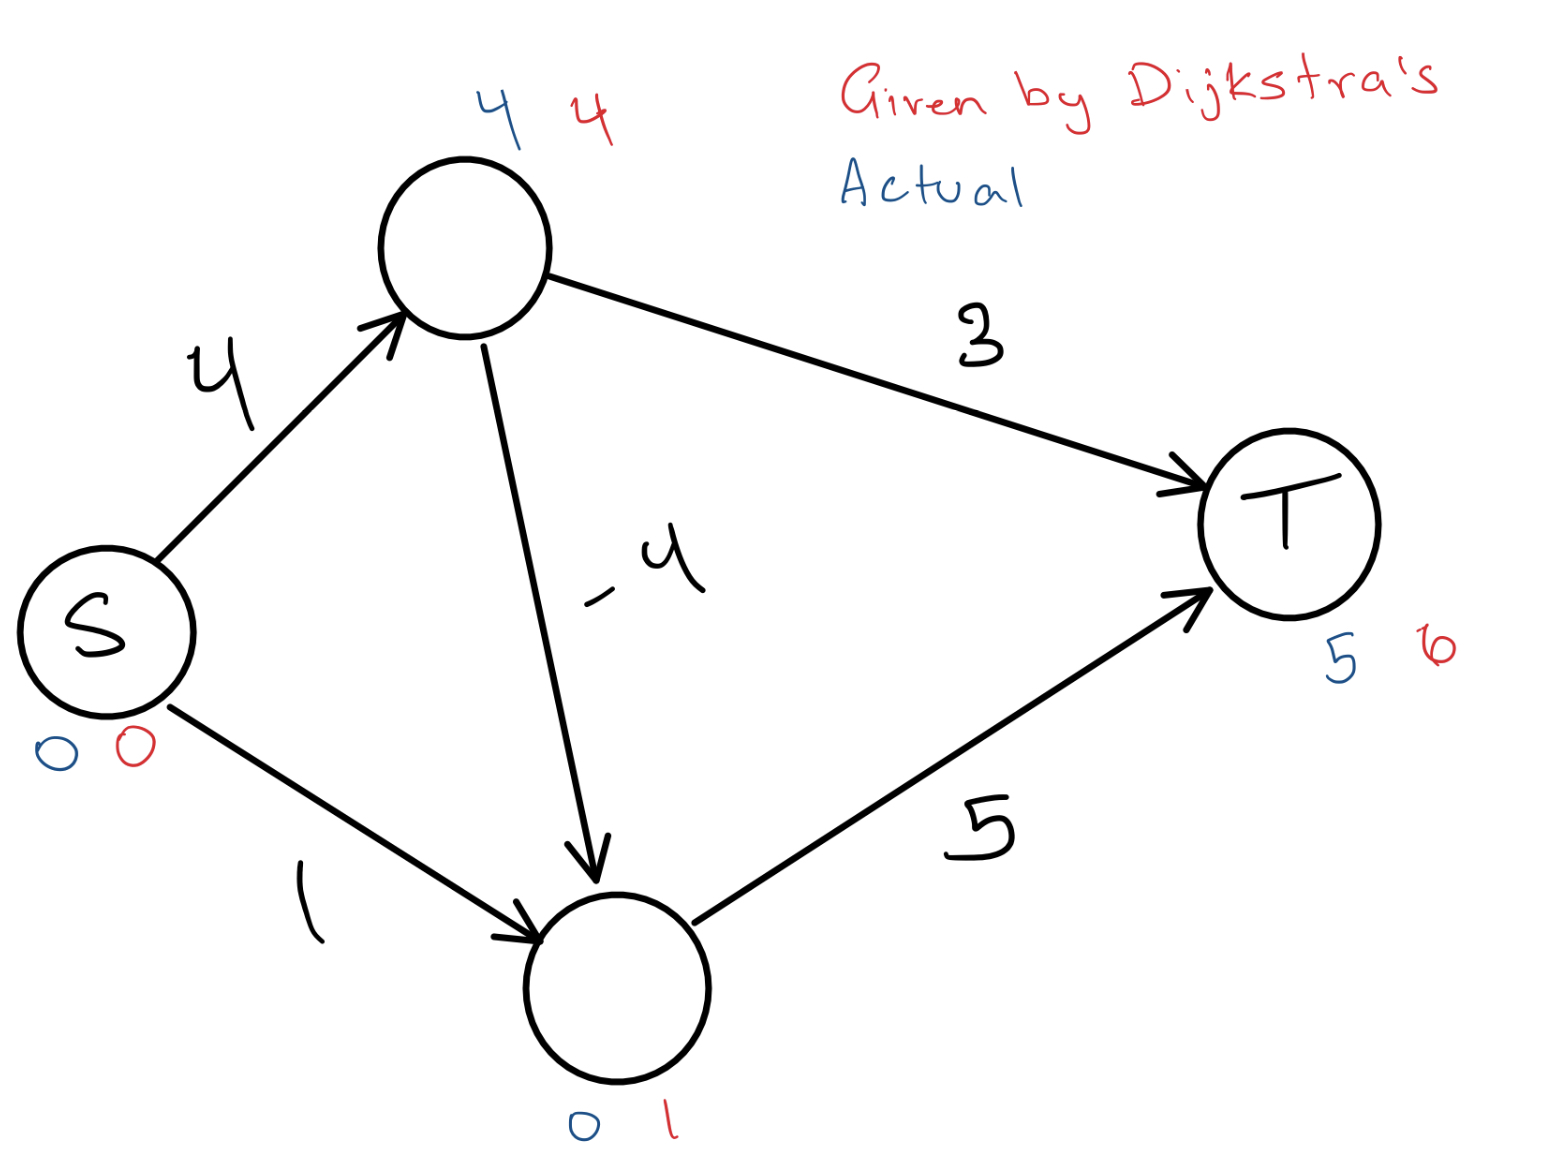
\includegraphics[scale=0.2]{s.jpeg}

    b)

    The termination of the while loop is that the heap is empty. Every single time the loop runs, the vertex that has the minimum distance is removed from H. In the event of a negative edge going to a node that has already been removed, it will update the distance of that already removed node, but it will not update the rest of the nodes that come after the removed node because it will never be visited in the loop again.

\end{document}
